\newpage
\begin{song}{title={Stary wrak}, music={Mechanicy Szanty}}
\small
    \begin{intro}
        \writechord{d} \writechord{a} \\
        \writechord{C} \writechord{D}\writechord{G} \\
        \writechord{a} \writechord{G} \writechord{asus2}
    \end{intro}
    \begin{multicols}{2}
    \begin{verse}
        Już za^{d}kończył życie swe ^{a} \\
        Oparł ^{C}dziób o stro^{D}my ^{G}brzeg \\
        Rejsu ^{a}kres wyznaczył cz^{G}as i morza gniew ^{asus2} \\
        Już pozostał tylko ślad \\
        Żagli, które targał wiatr \\
        Nie zawiodą go już więcej na swój szlak \\
        \\
        Tam gdzieś ^{a}czeka na nas znów \\
        Żagli ^{G}biel i silny wiatr \\
        Tam gdzieś ^{a}czeka żywioł, który wciąż nas ^{F}gna \\
        Gdzieś do ^{d}postrzępionych pa^{a}lm \\
        Do mil^{C}czących, zło^{D}tych ^{G}plaż \\
        Stary ^{a}wrak na pokład j^{G}uż nie weźmie nas ^{asus2}
    \end{verse}
    \begin{center}
        \vspace{0.6cm}
        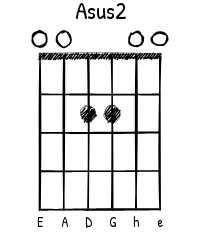
\includegraphics[height=3.5cm]{images/Asus2.png}
    \end{center}
    \vfill\null\columnbreak{}
    \begin{verse}
        Dzielny był przez tyle lat \\
        ``Czarnej Kuli'' nosił znak \\
        Imię jego wśród liniowców każdy znał \\
        Gdy na cumach w porcie stał \\
        Smukłe linie, piękny kształt \\
        Każdy morze razem z nim zdobywać chciał \\
        \\
        Płynąć tam, gdzie czeka znów \\
        Żagli biel i silny wiatr \\
        Płynąć tam, gdzie żywioł, który wciąż nas gna \\
        Gdzieś do postrzępionych palm \\
        Do milczących, złotych plaż \\
        Dziś na pokład stary wrak nie weźmie nas
    \end{verse}
    \begin{verse}
        To wędrówki jego kres \\
        Skończył się już żagli wiek \\
        Nie powrócą pod błękitny nieba dach \\
        Tylko w sercach naszych trwa \\
        Do żaglowców z tamtych lat \\
        Wielka miłość, która w morze ciągnie nas \\
        \\
        Chcemy płynąć tam, gdzie znów \\
        Żagli biel i silny wiatr \\
        Chcemy płynąć w żywioł, który wciąż nas gna \\
        Tam do postrzępionych palm \\
        Do milczących, złotych plaż \\
        Stary wrak wciąż pływać będzie w naszych snach
    \end{verse}
    \begin{interlude}
        Tam do postrzępionych palm \\
        Do milczących, złotych plaż \\
        Stary wrak wciąż pływać będzie w naszych snach
    \end{interlude}
    \end{multicols}
\end{song}

